% Created by tikzDevice version 0.12.3.1 on 2021-12-15 17:50:46
% !TEX encoding = UTF-8 Unicode
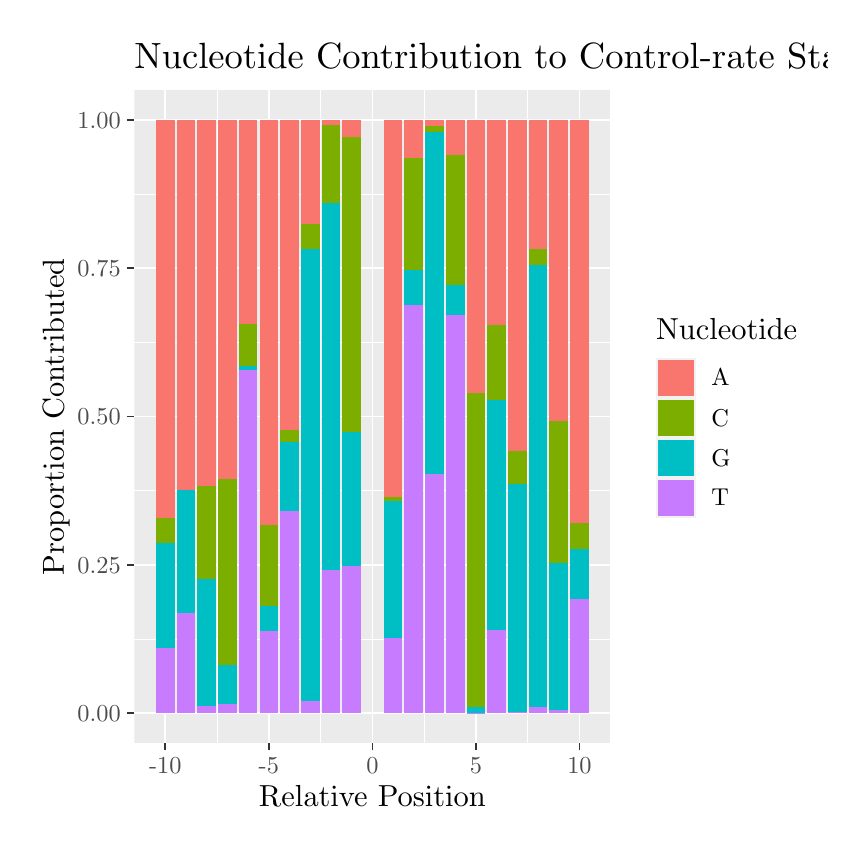
\begin{tikzpicture}[x=1pt,y=1pt]
\definecolor{fillColor}{RGB}{255,255,255}
\path[use as bounding box,fill=fillColor,fill opacity=0.00] (0,0) rectangle (289.08,289.08);
\begin{scope}
\path[clip] (  0.00,  0.00) rectangle (289.08,289.08);
\definecolor{drawColor}{RGB}{255,255,255}
\definecolor{fillColor}{RGB}{255,255,255}

\path[draw=drawColor,line width= 0.6pt,line join=round,line cap=round,fill=fillColor] (  0.00,  0.00) rectangle (289.08,289.08);
\end{scope}
\begin{scope}
\path[clip] ( 38.56, 30.69) rectangle (210.56,266.42);
\definecolor{fillColor}{gray}{0.92}

\path[fill=fillColor] ( 38.56, 30.69) rectangle (210.56,266.42);
\definecolor{drawColor}{RGB}{255,255,255}

\path[draw=drawColor,line width= 0.3pt,line join=round] ( 38.56, 68.19) --
	(210.56, 68.19);

\path[draw=drawColor,line width= 0.3pt,line join=round] ( 38.56,121.77) --
	(210.56,121.77);

\path[draw=drawColor,line width= 0.3pt,line join=round] ( 38.56,175.34) --
	(210.56,175.34);

\path[draw=drawColor,line width= 0.3pt,line join=round] ( 38.56,228.92) --
	(210.56,228.92);

\path[draw=drawColor,line width= 0.3pt,line join=round] ( 68.45, 30.69) --
	( 68.45,266.42);

\path[draw=drawColor,line width= 0.3pt,line join=round] (105.85, 30.69) --
	(105.85,266.42);

\path[draw=drawColor,line width= 0.3pt,line join=round] (143.26, 30.69) --
	(143.26,266.42);

\path[draw=drawColor,line width= 0.3pt,line join=round] (180.67, 30.69) --
	(180.67,266.42);

\path[draw=drawColor,line width= 0.6pt,line join=round] ( 38.56, 41.40) --
	(210.56, 41.40);

\path[draw=drawColor,line width= 0.6pt,line join=round] ( 38.56, 94.98) --
	(210.56, 94.98);

\path[draw=drawColor,line width= 0.6pt,line join=round] ( 38.56,148.55) --
	(210.56,148.55);

\path[draw=drawColor,line width= 0.6pt,line join=round] ( 38.56,202.13) --
	(210.56,202.13);

\path[draw=drawColor,line width= 0.6pt,line join=round] ( 38.56,255.71) --
	(210.56,255.71);

\path[draw=drawColor,line width= 0.6pt,line join=round] ( 49.74, 30.69) --
	( 49.74,266.42);

\path[draw=drawColor,line width= 0.6pt,line join=round] ( 87.15, 30.69) --
	( 87.15,266.42);

\path[draw=drawColor,line width= 0.6pt,line join=round] (124.56, 30.69) --
	(124.56,266.42);

\path[draw=drawColor,line width= 0.6pt,line join=round] (161.97, 30.69) --
	(161.97,266.42);

\path[draw=drawColor,line width= 0.6pt,line join=round] (199.38, 30.69) --
	(199.38,266.42);
\definecolor{fillColor}{RGB}{248,118,109}

\path[fill=fillColor] ( 46.37,111.76) rectangle ( 53.11,255.71);
\definecolor{fillColor}{RGB}{124,174,0}

\path[fill=fillColor] ( 46.37,102.73) rectangle ( 53.11,111.76);
\definecolor{fillColor}{RGB}{0,191,196}

\path[fill=fillColor] ( 46.37, 64.78) rectangle ( 53.11,102.73);
\definecolor{fillColor}{RGB}{199,124,255}

\path[fill=fillColor] ( 46.37, 41.40) rectangle ( 53.11, 64.78);
\definecolor{fillColor}{RGB}{248,118,109}

\path[fill=fillColor] ( 53.86,122.14) rectangle ( 60.59,255.71);
\definecolor{fillColor}{RGB}{124,174,0}

\path[fill=fillColor] ( 53.86,121.97) rectangle ( 60.59,122.14);
\definecolor{fillColor}{RGB}{0,191,196}

\path[fill=fillColor] ( 53.86, 77.74) rectangle ( 60.59,121.97);
\definecolor{fillColor}{RGB}{199,124,255}

\path[fill=fillColor] ( 53.86, 41.40) rectangle ( 60.59, 77.74);
\definecolor{fillColor}{RGB}{248,118,109}

\path[fill=fillColor] ( 61.34,123.52) rectangle ( 68.07,255.71);
\definecolor{fillColor}{RGB}{124,174,0}

\path[fill=fillColor] ( 61.34, 89.95) rectangle ( 68.07,123.52);
\definecolor{fillColor}{RGB}{0,191,196}

\path[fill=fillColor] ( 61.34, 43.89) rectangle ( 68.07, 89.95);
\definecolor{fillColor}{RGB}{199,124,255}

\path[fill=fillColor] ( 61.34, 41.40) rectangle ( 68.07, 43.89);
\definecolor{fillColor}{RGB}{248,118,109}

\path[fill=fillColor] ( 68.82,126.03) rectangle ( 75.55,255.71);
\definecolor{fillColor}{RGB}{124,174,0}

\path[fill=fillColor] ( 68.82, 58.79) rectangle ( 75.55,126.03);
\definecolor{fillColor}{RGB}{0,191,196}

\path[fill=fillColor] ( 68.82, 44.56) rectangle ( 75.55, 58.79);
\definecolor{fillColor}{RGB}{199,124,255}

\path[fill=fillColor] ( 68.82, 41.40) rectangle ( 75.55, 44.56);
\definecolor{fillColor}{RGB}{248,118,109}

\path[fill=fillColor] ( 76.30,181.95) rectangle ( 83.04,255.71);
\definecolor{fillColor}{RGB}{124,174,0}

\path[fill=fillColor] ( 76.30,166.75) rectangle ( 83.04,181.95);
\definecolor{fillColor}{RGB}{0,191,196}

\path[fill=fillColor] ( 76.30,165.48) rectangle ( 83.04,166.75);
\definecolor{fillColor}{RGB}{199,124,255}

\path[fill=fillColor] ( 76.30, 41.40) rectangle ( 83.04,165.48);
\definecolor{fillColor}{RGB}{248,118,109}

\path[fill=fillColor] ( 83.78,109.54) rectangle ( 90.52,255.71);
\definecolor{fillColor}{RGB}{124,174,0}

\path[fill=fillColor] ( 83.78, 79.92) rectangle ( 90.52,109.54);
\definecolor{fillColor}{RGB}{199,124,255}

\path[fill=fillColor] ( 83.78, 41.40) rectangle ( 90.52, 70.98);
\definecolor{fillColor}{RGB}{0,191,196}

\path[fill=fillColor] ( 83.78, 70.98) rectangle ( 90.52, 79.92);
\definecolor{fillColor}{RGB}{248,118,109}

\path[fill=fillColor] ( 91.27,143.79) rectangle ( 98.00,255.71);
\definecolor{fillColor}{RGB}{124,174,0}

\path[fill=fillColor] ( 91.27,139.49) rectangle ( 98.00,143.79);
\definecolor{fillColor}{RGB}{0,191,196}

\path[fill=fillColor] ( 91.27,114.37) rectangle ( 98.00,139.49);
\definecolor{fillColor}{RGB}{199,124,255}

\path[fill=fillColor] ( 91.27, 41.40) rectangle ( 98.00,114.37);
\definecolor{fillColor}{RGB}{248,118,109}

\path[fill=fillColor] ( 98.75,217.96) rectangle (105.48,255.71);
\definecolor{fillColor}{RGB}{124,174,0}

\path[fill=fillColor] ( 98.75,209.20) rectangle (105.48,217.96);
\definecolor{fillColor}{RGB}{0,191,196}

\path[fill=fillColor] ( 98.75, 45.72) rectangle (105.48,209.20);
\definecolor{fillColor}{RGB}{199,124,255}

\path[fill=fillColor] ( 98.75, 41.40) rectangle (105.48, 45.72);
\definecolor{fillColor}{RGB}{248,118,109}

\path[fill=fillColor] (106.23,253.84) rectangle (112.96,255.71);
\definecolor{fillColor}{RGB}{124,174,0}

\path[fill=fillColor] (106.23,225.64) rectangle (112.96,253.84);
\definecolor{fillColor}{RGB}{199,124,255}

\path[fill=fillColor] (106.23, 41.40) rectangle (112.96, 93.09);
\definecolor{fillColor}{RGB}{0,191,196}

\path[fill=fillColor] (106.23, 93.09) rectangle (112.96,225.64);
\definecolor{fillColor}{RGB}{248,118,109}

\path[fill=fillColor] (113.71,249.52) rectangle (120.44,255.71);
\definecolor{fillColor}{RGB}{124,174,0}

\path[fill=fillColor] (113.71,143.01) rectangle (120.44,249.52);
\definecolor{fillColor}{RGB}{0,191,196}

\path[fill=fillColor] (113.71, 94.59) rectangle (120.44,143.01);
\definecolor{fillColor}{RGB}{199,124,255}

\path[fill=fillColor] (113.71, 41.40) rectangle (120.44, 94.59);
\definecolor{fillColor}{RGB}{248,118,109}

\path[fill=fillColor] (128.67,119.31) rectangle (135.41,255.71);
\definecolor{fillColor}{RGB}{124,174,0}

\path[fill=fillColor] (128.67,118.18) rectangle (135.41,119.31);
\definecolor{fillColor}{RGB}{0,191,196}

\path[fill=fillColor] (128.67, 68.59) rectangle (135.41,118.18);
\definecolor{fillColor}{RGB}{199,124,255}

\path[fill=fillColor] (128.67, 41.40) rectangle (135.41, 68.59);
\definecolor{fillColor}{RGB}{248,118,109}

\path[fill=fillColor] (136.16,241.99) rectangle (142.89,255.71);
\definecolor{fillColor}{RGB}{124,174,0}

\path[fill=fillColor] (136.16,201.42) rectangle (142.89,241.99);
\definecolor{fillColor}{RGB}{199,124,255}

\path[fill=fillColor] (136.16, 41.40) rectangle (142.89,189.03);
\definecolor{fillColor}{RGB}{0,191,196}

\path[fill=fillColor] (136.16,189.03) rectangle (142.89,201.42);
\definecolor{fillColor}{RGB}{248,118,109}

\path[fill=fillColor] (143.64,253.48) rectangle (150.37,255.71);
\definecolor{fillColor}{RGB}{124,174,0}

\path[fill=fillColor] (143.64,251.53) rectangle (150.37,253.48);
\definecolor{fillColor}{RGB}{0,191,196}

\path[fill=fillColor] (143.64,127.83) rectangle (150.37,251.53);
\definecolor{fillColor}{RGB}{199,124,255}

\path[fill=fillColor] (143.64, 41.40) rectangle (150.37,127.83);
\definecolor{fillColor}{RGB}{248,118,109}

\path[fill=fillColor] (151.12,243.12) rectangle (157.85,255.71);
\definecolor{fillColor}{RGB}{124,174,0}

\path[fill=fillColor] (151.12,196.17) rectangle (157.85,243.12);
\definecolor{fillColor}{RGB}{0,191,196}

\path[fill=fillColor] (151.12,185.23) rectangle (157.85,196.17);
\definecolor{fillColor}{RGB}{199,124,255}

\path[fill=fillColor] (151.12, 41.40) rectangle (157.85,185.23);
\definecolor{fillColor}{RGB}{248,118,109}

\path[fill=fillColor] (158.60,157.13) rectangle (165.34,255.71);
\definecolor{fillColor}{RGB}{124,174,0}

\path[fill=fillColor] (158.60, 43.74) rectangle (165.34,157.13);
\definecolor{fillColor}{RGB}{0,191,196}

\path[fill=fillColor] (158.60, 41.42) rectangle (165.34, 43.74);
\definecolor{fillColor}{RGB}{199,124,255}

\path[fill=fillColor] (158.60, 41.40) rectangle (165.34, 41.42);
\definecolor{fillColor}{RGB}{248,118,109}

\path[fill=fillColor] (166.08,181.61) rectangle (172.82,255.71);
\definecolor{fillColor}{RGB}{124,174,0}

\path[fill=fillColor] (166.08,154.51) rectangle (172.82,181.61);
\definecolor{fillColor}{RGB}{0,191,196}

\path[fill=fillColor] (166.08, 71.42) rectangle (172.82,154.51);
\definecolor{fillColor}{RGB}{199,124,255}

\path[fill=fillColor] (166.08, 41.40) rectangle (172.82, 71.42);
\definecolor{fillColor}{RGB}{248,118,109}

\path[fill=fillColor] (173.57,136.21) rectangle (180.30,255.71);
\definecolor{fillColor}{RGB}{124,174,0}

\path[fill=fillColor] (173.57,124.05) rectangle (180.30,136.21);
\definecolor{fillColor}{RGB}{199,124,255}

\path[fill=fillColor] (173.57, 41.40) rectangle (180.30, 41.97);
\definecolor{fillColor}{RGB}{0,191,196}

\path[fill=fillColor] (173.57, 41.97) rectangle (180.30,124.05);
\definecolor{fillColor}{RGB}{248,118,109}

\path[fill=fillColor] (181.05,209.11) rectangle (187.78,255.71);
\definecolor{fillColor}{RGB}{124,174,0}

\path[fill=fillColor] (181.05,203.23) rectangle (187.78,209.11);
\definecolor{fillColor}{RGB}{0,191,196}

\path[fill=fillColor] (181.05, 43.75) rectangle (187.78,203.23);
\definecolor{fillColor}{RGB}{199,124,255}

\path[fill=fillColor] (181.05, 41.40) rectangle (187.78, 43.75);
\definecolor{fillColor}{RGB}{248,118,109}

\path[fill=fillColor] (188.53,146.96) rectangle (195.26,255.71);
\definecolor{fillColor}{RGB}{124,174,0}

\path[fill=fillColor] (188.53, 95.75) rectangle (195.26,146.96);
\definecolor{fillColor}{RGB}{0,191,196}

\path[fill=fillColor] (188.53, 42.67) rectangle (195.26, 95.75);
\definecolor{fillColor}{RGB}{199,124,255}

\path[fill=fillColor] (188.53, 41.40) rectangle (195.26, 42.67);
\definecolor{fillColor}{RGB}{248,118,109}

\path[fill=fillColor] (196.01,109.92) rectangle (202.75,255.71);
\definecolor{fillColor}{RGB}{124,174,0}

\path[fill=fillColor] (196.01,100.62) rectangle (202.75,109.92);
\definecolor{fillColor}{RGB}{0,191,196}

\path[fill=fillColor] (196.01, 82.47) rectangle (202.75,100.62);
\definecolor{fillColor}{RGB}{199,124,255}

\path[fill=fillColor] (196.01, 41.40) rectangle (202.75, 82.47);
\end{scope}
\begin{scope}
\path[clip] (  0.00,  0.00) rectangle (289.08,289.08);
\definecolor{drawColor}{gray}{0.30}

\node[text=drawColor,anchor=base east,inner sep=0pt, outer sep=0pt, scale=  0.88] at ( 33.61, 38.37) {0.00};

\node[text=drawColor,anchor=base east,inner sep=0pt, outer sep=0pt, scale=  0.88] at ( 33.61, 91.95) {0.25};

\node[text=drawColor,anchor=base east,inner sep=0pt, outer sep=0pt, scale=  0.88] at ( 33.61,145.52) {0.50};

\node[text=drawColor,anchor=base east,inner sep=0pt, outer sep=0pt, scale=  0.88] at ( 33.61,199.10) {0.75};

\node[text=drawColor,anchor=base east,inner sep=0pt, outer sep=0pt, scale=  0.88] at ( 33.61,252.68) {1.00};
\end{scope}
\begin{scope}
\path[clip] (  0.00,  0.00) rectangle (289.08,289.08);
\definecolor{drawColor}{gray}{0.20}

\path[draw=drawColor,line width= 0.6pt,line join=round] ( 35.81, 41.40) --
	( 38.56, 41.40);

\path[draw=drawColor,line width= 0.6pt,line join=round] ( 35.81, 94.98) --
	( 38.56, 94.98);

\path[draw=drawColor,line width= 0.6pt,line join=round] ( 35.81,148.55) --
	( 38.56,148.55);

\path[draw=drawColor,line width= 0.6pt,line join=round] ( 35.81,202.13) --
	( 38.56,202.13);

\path[draw=drawColor,line width= 0.6pt,line join=round] ( 35.81,255.71) --
	( 38.56,255.71);
\end{scope}
\begin{scope}
\path[clip] (  0.00,  0.00) rectangle (289.08,289.08);
\definecolor{drawColor}{gray}{0.20}

\path[draw=drawColor,line width= 0.6pt,line join=round] ( 49.74, 27.94) --
	( 49.74, 30.69);

\path[draw=drawColor,line width= 0.6pt,line join=round] ( 87.15, 27.94) --
	( 87.15, 30.69);

\path[draw=drawColor,line width= 0.6pt,line join=round] (124.56, 27.94) --
	(124.56, 30.69);

\path[draw=drawColor,line width= 0.6pt,line join=round] (161.97, 27.94) --
	(161.97, 30.69);

\path[draw=drawColor,line width= 0.6pt,line join=round] (199.38, 27.94) --
	(199.38, 30.69);
\end{scope}
\begin{scope}
\path[clip] (  0.00,  0.00) rectangle (289.08,289.08);
\definecolor{drawColor}{gray}{0.30}

\node[text=drawColor,anchor=base,inner sep=0pt, outer sep=0pt, scale=  0.88] at ( 49.74, 19.68) {-10};

\node[text=drawColor,anchor=base,inner sep=0pt, outer sep=0pt, scale=  0.88] at ( 87.15, 19.68) {-5};

\node[text=drawColor,anchor=base,inner sep=0pt, outer sep=0pt, scale=  0.88] at (124.56, 19.68) {0};

\node[text=drawColor,anchor=base,inner sep=0pt, outer sep=0pt, scale=  0.88] at (161.97, 19.68) {5};

\node[text=drawColor,anchor=base,inner sep=0pt, outer sep=0pt, scale=  0.88] at (199.38, 19.68) {10};
\end{scope}
\begin{scope}
\path[clip] (  0.00,  0.00) rectangle (289.08,289.08);
\definecolor{drawColor}{RGB}{0,0,0}

\node[text=drawColor,anchor=base,inner sep=0pt, outer sep=0pt, scale=  1.10] at (124.56,  7.64) {Relative Position};
\end{scope}
\begin{scope}
\path[clip] (  0.00,  0.00) rectangle (289.08,289.08);
\definecolor{drawColor}{RGB}{0,0,0}

\node[text=drawColor,rotate= 90.00,anchor=base,inner sep=0pt, outer sep=0pt, scale=  1.10] at ( 13.08,148.55) {Proportion Contributed};
\end{scope}
\begin{scope}
\path[clip] (  0.00,  0.00) rectangle (289.08,289.08);
\definecolor{fillColor}{RGB}{255,255,255}

\path[fill=fillColor] (221.56,106.54) rectangle (283.58,190.57);
\end{scope}
\begin{scope}
\path[clip] (  0.00,  0.00) rectangle (289.08,289.08);
\definecolor{drawColor}{RGB}{0,0,0}

\node[text=drawColor,anchor=base west,inner sep=0pt, outer sep=0pt, scale=  1.10] at (227.06,176.42) {Nucleotide};
\end{scope}
\begin{scope}
\path[clip] (  0.00,  0.00) rectangle (289.08,289.08);
\definecolor{fillColor}{gray}{0.95}

\path[fill=fillColor] (227.06,155.40) rectangle (241.52,169.86);
\end{scope}
\begin{scope}
\path[clip] (  0.00,  0.00) rectangle (289.08,289.08);
\definecolor{fillColor}{RGB}{248,118,109}

\path[fill=fillColor] (227.78,156.11) rectangle (240.81,169.14);
\end{scope}
\begin{scope}
\path[clip] (  0.00,  0.00) rectangle (289.08,289.08);
\definecolor{fillColor}{gray}{0.95}

\path[fill=fillColor] (227.06,140.95) rectangle (241.52,155.40);
\end{scope}
\begin{scope}
\path[clip] (  0.00,  0.00) rectangle (289.08,289.08);
\definecolor{fillColor}{RGB}{124,174,0}

\path[fill=fillColor] (227.78,141.66) rectangle (240.81,154.69);
\end{scope}
\begin{scope}
\path[clip] (  0.00,  0.00) rectangle (289.08,289.08);
\definecolor{fillColor}{gray}{0.95}

\path[fill=fillColor] (227.06,126.49) rectangle (241.52,140.95);
\end{scope}
\begin{scope}
\path[clip] (  0.00,  0.00) rectangle (289.08,289.08);
\definecolor{fillColor}{RGB}{0,191,196}

\path[fill=fillColor] (227.78,127.20) rectangle (240.81,140.24);
\end{scope}
\begin{scope}
\path[clip] (  0.00,  0.00) rectangle (289.08,289.08);
\definecolor{fillColor}{gray}{0.95}

\path[fill=fillColor] (227.06,112.04) rectangle (241.52,126.49);
\end{scope}
\begin{scope}
\path[clip] (  0.00,  0.00) rectangle (289.08,289.08);
\definecolor{fillColor}{RGB}{199,124,255}

\path[fill=fillColor] (227.78,112.75) rectangle (240.81,125.78);
\end{scope}
\begin{scope}
\path[clip] (  0.00,  0.00) rectangle (289.08,289.08);
\definecolor{drawColor}{RGB}{0,0,0}

\node[text=drawColor,anchor=base west,inner sep=0pt, outer sep=0pt, scale=  0.88] at (247.02,159.60) {A};
\end{scope}
\begin{scope}
\path[clip] (  0.00,  0.00) rectangle (289.08,289.08);
\definecolor{drawColor}{RGB}{0,0,0}

\node[text=drawColor,anchor=base west,inner sep=0pt, outer sep=0pt, scale=  0.88] at (247.02,145.14) {C};
\end{scope}
\begin{scope}
\path[clip] (  0.00,  0.00) rectangle (289.08,289.08);
\definecolor{drawColor}{RGB}{0,0,0}

\node[text=drawColor,anchor=base west,inner sep=0pt, outer sep=0pt, scale=  0.88] at (247.02,130.69) {G};
\end{scope}
\begin{scope}
\path[clip] (  0.00,  0.00) rectangle (289.08,289.08);
\definecolor{drawColor}{RGB}{0,0,0}

\node[text=drawColor,anchor=base west,inner sep=0pt, outer sep=0pt, scale=  0.88] at (247.02,116.24) {T};
\end{scope}
\begin{scope}
\path[clip] (  0.00,  0.00) rectangle (289.08,289.08);
\definecolor{drawColor}{RGB}{0,0,0}

\node[text=drawColor,anchor=base west,inner sep=0pt, outer sep=0pt, scale=  1.32] at ( 38.56,274.49) {Nucleotide Contribution to Control-rate Statistic: AT-CG};
\end{scope}
\end{tikzpicture}
